\documentclass[12pt]{article}
\usepackage{natbib,amsmath,amsfonts,fullpage,hyphenat,booktabs,graphicx,setspace}
\usepackage[colorlinks,linkcolor=blue,citecolor=blue,urlcolor=blue]{hyperref}
\setcitestyle{square,super,comma}
\onehalfspacing{}

\title{Architecture and agent definition\\Multiagent and Agent System}
\author{Arun Prabhu\\Md Zahiduzzaman\\Dharmin Bakaraniya}
\begin{document}
\maketitle{}
\pagebreak
\section{Architecture}%
\label{sec:architecture}

\begin{figure}[htpb]
    \centering
    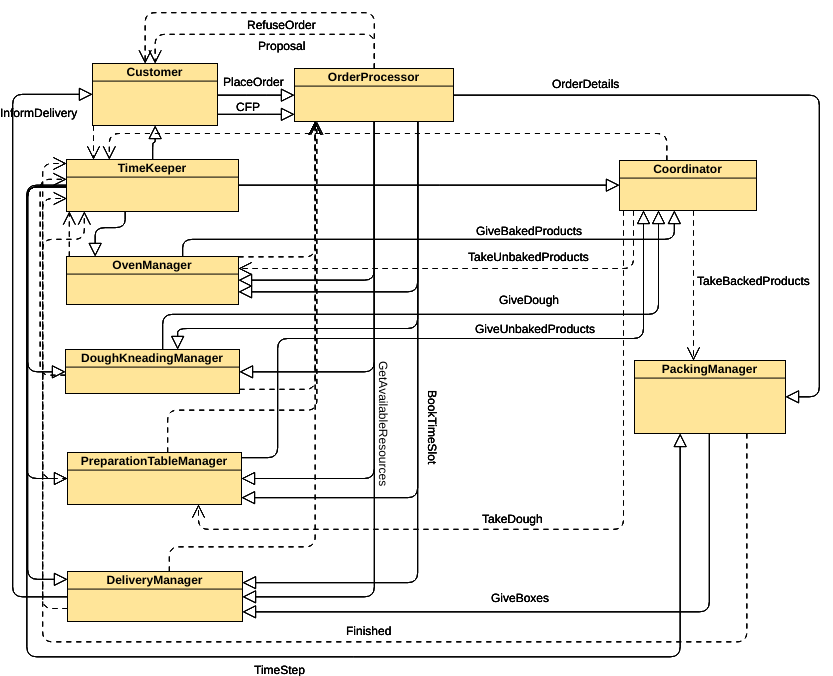
\includegraphics[width=1.0\linewidth]{Bakery.png}
    \caption{Architecture diagram explaining the interaction between customer and bakery agents}\label{fig:somename}
\end{figure}

\pagebreak

\section{Architectural Description}%
\label{sec:description}
We implement a quasi-distributed approach to develop this architecture instead of going completely distributed. This enables easier planning. It also enables us to loosely follow the Single Responsibility principle. Ex : Anything related to Ovens is taken care by OvenManager and so on.
\begin{itemize}
    \item \textbf{Customer}: It is quite obvious that each customer needs to be assigned an Agent. This type of Agents are spawned based on the meta.json file (which contains details about customers) at the beginning by the TimeKeeper. The Agent is terminated at the end of simulation when the TimeKeeper initiates a platform shutdown. It interacts with OrderProcessor in two ways.,
    \begin{enumerate}
    	\item To ask for product proposals.
    	\item To place order. 
    \end{enumerate}
    For the prior the OrderProcessor responds with a proposal and for the later it responds with a refuse order if it cannot be taken up by the bakery in the stipulated time or if it does not make that type of product.
    \item \textbf{OrderProcessor}: OrderProcessor can be considered as the first Agent for every bakery. The responsibility of this Agent is to interact with the customer Agent. It also interacts with the other Agents in the bakery (OvenManager, DoughKneadingManager, PreparationTableManager, DeliveryManager) to check for the available resources before it can confirm the order with the customer. It also interacts with the PackingManager to provide it with the order details for packing.
    \item \textbf{TimeKeeper}: This is the first Agent which is spawned. It is responsible for the movement of time in the entire bakery eco-system. This is responsible for providing all the other agents with a common time reference so that everyone are in sync. This also gets feedback from all the agents about the status of their tasks. If all the agents are done with whatever task they were supposed to finish in the time step, the TimeKeeper increments the time step. It is also responsible for shutting down the platform when the simulation time ends.
    \item \textbf{OvenManager}: We assign a single Agent to manage all the ovens in the bakery. This manager acts like a point of contact for all queries related to ovens and baking. The status about the availability of free trays, cooling times and heating times of different products are entirely kept track by this agent. It interacts with the OrderProcessor during order taking, to provide the status of the availability of the free trays in the ovens. If a new order is confirmed, a request to book the timeslot is also recieved from the OrderProcessor. It also interacts with the Coordinator Agent (Interface between Baking and Packing stages) and provides it with the baked products after they have been cooled.
    \item \textbf{DoughKneadingManager}: We assign a single Agent to manage the entire dough kneading process. This manager acts like a point of contact for all queries related to kneading machine and raw dough. It interacts with the OrderProcessor during order taking, to provide the status of the availability of the kneading machine. If a new order is confirmed, a request to book the timeslot is also recieved from the Order Processor. It also interacts with the Coordinator Agent(Interface between Dough preparation and Product preparation stages) and provides it with the kneaded dough after the resting time is over.
    \item \textbf{PreparationTableManager}: We assign a single Agent to manage the product preparation process. This manager acts like a point of contact for all queries related to product preparation. It interacts with the OrderProcessor during order taking, to provide the status of the availability of the Preparation Tables. If a new order is confirmed, a request to book the timeslot is also recieved from the Order Processor. It also interacts with the Coordinator Agent(Interface between Product preparation and Baking stages) and provides it with the unbaked products after they have been prepared.
    \item \textbf{PackingManager}: We assign a single Agent to manage the packing process. This manager interacts with the OrderProcessor to get the order details. It interacts with the Coordinator Agent (Interface between Baking and Packing stages) which provides it with the baked and cooled products for packing. It also interacts with the Delivery Manager by providing it with Packed boxes for delivery.
    \item \textbf{DeliveryManager}: We assign a single Agent to manage the logistic process. This manager interacts with the OrderProcessor during order taking, to provide the status of the availability of the trucks for delivery. If a new order is confirmed, a request to book the timeslot is also recieved from the Order Processor. It receives the packed products to deliver, from the PackingManager. The delivery manager also informs the customer about the successful delivery of order.
    \item \textbf{Coordinator}: This is a general type of Agent with acts as an iterface between various stages in the bakery. We spawn three agents of this type to serve the following roles,
    \begin{enumerate}
    \item Interface between Baking and Packing stages.
    \item Interface between Product preparation and Baking.
    \item Interface between Dough preparation and Product preparation.
    \end{enumerate}
\end{itemize}


\section{Class descriptions}%
\label{sec:agent_descriptions}

\subsection{Customer}%
\label{sub:customer_agent}
\begin{itemize}
    \item \textbf{Stage}: Order
    \item \textbf{Agent/Object}: Agent
    \item \textbf{Static/Dynamic}: Static
    \item \textbf{Behaviour}: PlaceOrder (Generic)
    \item \textbf{Messages in}:
        \begin{itemize}
            \item AskForPriceProposal (Sender: OrderProcessor)
            \item AskForPriceRefuse (Sender: OrderProcessor)
            \item RefuseOrder (Sender: OrderProcessor)
            \item TimeStep (Sender: Time Keeper)
        \end{itemize}
    \item \textbf{Messages out}:
        \begin{itemize}
            \item AskForPrice (Receiver: OrderProcessor)
            \item PlaceOrder (Receiver: OrderProcessor)
            \item Finished (Receiver: Time Keeper)
        \end{itemize}
\end{itemize}

\newpage{}
\subsection{Order Processor}%
\label{sub:order_processor}
\begin{itemize}
    \item \textbf{Stage}: Order
    \item \textbf{Agent/Object}: Agent
    \item \textbf{Static/Dynamic}: Static
    \item \textbf{Behaviour}: CFPServer (Cyclic), OrderServer (Cyclic)
    \item \textbf{Messages in}:
        \begin{itemize}
            \item AskForPrice (Sender: Customer)
            \item PlaceOrder (Sender: Customer)
            \item ResourceAvailabilityResponce (Sender: Oven Manager, Dough Kneading Manager, Prep Table Manager, Delivery Manager)
            \item TimeStep (Sender: Time Keeper)
        \end{itemize}
    \item \textbf{Messages out}:
        \begin{itemize}
            \item AskForPriceProposal (Receiver: Customer)
            \item AskForPriceRefuse (Receiver: Customer)
            \item ResourceAvailability (Receiver: Oven Manager, Dough Kneading Manager, Prep Table Manager, Delivery Manager)
            \item BookTimeSlot (Receiver: Oven Manager, Dough Kneading Manager, Prep Table Manager, Delivery Manager)
            \item OrderDetails (Receiver: Packaging Manager)
            \item Finished (Receiver: Time Keeper)
        \end{itemize}
\end{itemize}

\newpage{}
\subsection{Oven Manager}%
\label{sub:over_manager}
\begin{itemize}
    \item \textbf{Stage}: OrderProcessing
    \item \textbf{Agent/Object}: Agent
    \item \textbf{Static/Dynamic}: Static
    \item \textbf{Behaviour}: ResourceAvailabilityServer (Cyclic), BookingServer (Cyclic), Bake (Generic)
    \item \textbf{Message in}:
        \begin{itemize}
            \item ResourceAvailability (Sender: Order Processor)
            \item BookTimeSlot (Sender: Order Processor)
            \item UnbakedProducts (Sender: Coordinator)
            \item TimeStep (Sender: Time Keeper)
        \end{itemize}
    \item \textbf{Message out}:
        \begin{itemize}
            \item ResourceAvailabilityResponce (Receiver: OrderProcessor)
            \item RequestUnbackedProducts (Receiver: Coordinator)
            \item BakedProducts (Receiver: Coordinator)
            \item Finished (Receiver: Time Keeper)
        \end{itemize}
\end{itemize}

\newpage{}
\subsection{Dough Kneading Manager}%
\label{sub:knead_manager}
\begin{itemize}
    \item \textbf{Stage}: OrderProcessing
    \item \textbf{Agent/Object}: Agent
    \item \textbf{Static/Dynamic}: Static
    \item \textbf{Behaviour}: ResourceAvailabilityServer (Cyclic), BookingServer (Cyclic), Knead (Generic)
    \item \textbf{Message in}:
        \begin{itemize}
            \item ResourceAvailability (Sender: Order Processor)
            \item BookTimeSlot (Sender: Order Processor)
            \item TimeStep (Sender: Time Keeper)
        \end{itemize}
    \item \textbf{Message out}:
        \begin{itemize}
            \item ResourceAvailabilityResponce (Receiver: OrderProcessor)
            \item Dough (Receiver: Coordinator)
            \item Finished (Receiver: Time Keeper)
        \end{itemize}
\end{itemize}

\newpage{}
\subsection{Prep Table Manager}%
\label{sub:prep_manager}
\begin{itemize}
    \item \textbf{Stage}: OrderProcessing
    \item \textbf{Agent/Object}: Agent
    \item \textbf{Static/Dynamic}: Static
    \item \textbf{Behaviour}: ResourceAvailabilityServer (Cyclic), BookingServer (Cyclic), Prepare (Generic)
    \item \textbf{Message in}:
        \begin{itemize}
            \item ResourceAvailability (Sender: Order Processor)
            \item BookTimeSlot (Sender: Order Processor)
            \item Dough (Sender: Coordinator)
            \item TimeStep (Sender: Time Keeper)
        \end{itemize}
    \item \textbf{Message out}:
        \begin{itemize}
            \item ResourceAvailabilityResponce (Receiver: OrderProcessor)
            \item RequestDough (Receiver: Coordinator)
            \item UnbakedProducts (Receiver: Coordinator)
            \item Finished (Receiver: Time Keeper)
        \end{itemize}
\end{itemize}

\newpage{}
\subsection{Coordinator}%
\label{sub:idle_manager}
\begin{itemize}
    \item \textbf{Stage}: OrderProcessor
    \item \textbf{Agent/Object}: Agent
    \item \textbf{Static/Dynamic}: Static
    \item \textbf{Behaviour}: SetDough (Cyclic), GetDough (Cyclic), SetUnbakedProducts (Cyclic), GetUnbakedProducts (Cyclic), SetBakedProducts (Cyclic), GetBakedProducts (Cyclic)
    \item \textbf{Message in}:
        \begin{itemize}
            \item RequestUnbackedProducts (Sender: Oven Manager)
            \item UnbakedProducts (Sender: Prep Table Manager)
            \item RequestBakedProducts (Sender: Packaging Manager)
            \item BakedProducts (Sender: Oven Manager)
            \item RequestDough (Sender: Prep Table Manager)
            \item Dough (Sender: Kneading Manager)
            \item TimeStep (Sender: Time Keeper)
        \end{itemize}
    \item \textbf{Message out}:
        \begin{itemize}
            \item UnbakedProducts (Receiver: Oven Manager)
            \item BakedProducts   (Receiver: Packaging Manager)
            \item Dough           (Receiver: Prep Table Manager)
            \item Finished (Receiver: Time Keeper)
        \end{itemize}
\end{itemize}

\newpage{}
\subsection{Packaging Manager}%
\label{sub:packaging_manager}
\begin{itemize}
    \item \textbf{Stage}: OrderProcessing
    \item \textbf{Agent/Object}: Agent
    \item \textbf{Static/Dynamic}: Static
    \item \textbf{Behaviour}: OrderDetailsServer (Cyclic), Pack (Cyclic)
    \item \textbf{Message in}:
        \begin{itemize}
            \item OrderDetails (Sender: Order Processor)
            \item BakedProducts (Sender: Coordinator)
            \item TimeStep (Sender: Time Keeper)
        \end{itemize}
    \item \textbf{Message out}:
        \begin{itemize}
            \item RequestBakedProducts (Receiver: Coordinator)
            \item Boxes (Receiver: Delivery Manager)
            \item Finished (Receiver: Time Keeper)
        \end{itemize}
\end{itemize}

\newpage{}
\subsection{Delivery Manager}%
\label{sub:delivery_manager}
\begin{itemize}
    \item \textbf{Stage}: Delivery
    \item \textbf{Agent/Object}: Agent
    \item \textbf{Static/Dynamic}: Static
    \item \textbf{Behaviour}: ResourceAvailabilityServer (Cyclic), BookingServer (Cyclic), Deliver (Generic)
    \item \textbf{Message in}:
        \begin{itemize}
            \item ResourceAvailability (Sender: Order Processor)
            \item BookTimeSlot (Sender: Order Processor)
            \item Boxes (Sender: Packaging Manager)
            \item TimeStep (Sender: Time Keeper)
        \end{itemize}
    \item \textbf{Message out}:
        \begin{itemize}
            \item ResourceAvailabilityResponce (Receiver: OrderProcessor)
            \item InformDelivery (Receiver: Customer)
            \item Finished (Receiver: Time Keeper)
        \end{itemize}
\end{itemize}

\newpage{}
\subsection{Time Keeper}%
\label{sub:time_keeper}
\begin{itemize}
    \item \textbf{Stage}: Order, OrderProcessing, Delivery
    \item \textbf{Agent/Object}: Agent
    \item \textbf{Static/Dynamic}: Static
    \item \textbf{Behaviour}: Clock (Generic), Shutdown (One shot)
    \item \textbf{Message in}:
        \begin{itemize}
            \item Finished (Sender: All Agents)
        \end{itemize}
    \item \textbf{Message out}:
        \begin{itemize}
            \item TimeStep (Receiver: All Agents)
        \end{itemize}
    \item \textbf{Explantion about its working}:
        \begin{itemize}
            \item The \textbf{Clock} behaviour has two steps. Based on current status, one of the step will be executed.
            \item The first step is to send messages (\texttt{TimeStep}) to each and every alive agent. This will be INFORM type. This tells all the agent to perform the task they are supposed to do in that particular time step.
            \item Once they are done with any actions that they are supposed to perform in a particular time step, they will respond (\texttt{Finished}) with an INFORM message. Then they will wait for another \texttt{TimeStep} message before performing any actions.
            \item The second step is to wait for responce from all alive agents. Once it gets all the responce messages, it increaments the \texttt{currentTime} (which signifies the simulation time). 
            \item The \texttt{done} method checks if the \texttt{currentTime} is more than \texttt{endTime} (read from \texttt{meta.json}). If it is then it will call \texttt{Shutdown} behaviour otherwise it will execute first step.
        \end{itemize}
\end{itemize}

\newpage{}
\subsection{Order}%
\label{sub:order}
\begin{itemize}
    \item \textbf{Stage}: Order
    \item \textbf{Agent/Object}: Object
    \item \textbf{Static/Dynamic}: Static
\end{itemize}

\subsection{Truck}%
\label{sub:truck}
\begin{itemize}
    \item \textbf{Stage}: Delivery
    \item \textbf{Agent/Object}: Object
    \item \textbf{Static/Dynamic}: Static
\end{itemize}

\subsection{Product}%
\label{sub:product}
\begin{itemize}
    \item \textbf{Stage}: Order, OrderProcessing, Delivery
    \item \textbf{Agent/Object}: Object
    \item \textbf{Static/Dynamic}: Dynamic
\end{itemize}

\subsection{Location}%
\label{sub:location}
\begin{itemize}
    \item \textbf{Stage}: Delivery
    \item \textbf{Agent/Object}: Object
    \item \textbf{Static/Dynamic}: Dynamic
\end{itemize}

\subsection{StreetNetwork}%
\label{sub:street_network}
\begin{itemize}
    \item \textbf{Stage}: Delivery
    \item \textbf{Agent/Object}: Object
    \item \textbf{Static/Dynamic}: Static
\end{itemize}

\section{Order Aggregation}%
\begin{itemize}
    \item As mentioned in the slides, the expected order times are as follows,
    \begin{enumerate}
    	\item 50\% to 100\% of the orders from super markets and sales shops arrive at the end of the day before delivery. They are next day orders. The remaining orders $<$ 50\% orders from the super markets and sales shops arrive on the same day as delivery.
    	\item All the orders from hospitals and old age homes arrive once a day (might not be fixed time), but for next day delivery.
    	\item Some customers like catering services, clubs etc make orders several days ahead of delivery.
    \end{enumerate}
    \item To ensure freshness and the reputation of the bakery, products can only be produced on the day of the order (however the dough preparation should also be done on the same day or not is not mentioned so we assume there is no restriction on that.)
    \item With this overview in mind we can see that before the start of the shift, the information about the next day orders is already known and hence the dough preparation can be planned for all the orders combined as it is independent of the type of product to be made.
    \item From the orders which are received (at the end of the delivery) for the super markets for the next day delivery, we can approximate them to be around 75\% ((50+100)/2) of the total orders expected and we can assume that we might get another 25\% (100-75) of orders on the same day as delivery. This is just an \textbf{estimated guess}. 
    \item In reality, it might happen that,
    \begin{enumerate}
    \item the same day orders might be less than 25\% of the total next day orders. 
    \item sometimes they might be more than 25\% of the total next day orders. 
    \end{enumerate}
    \item For the prior case, the dough is already available. For the latter case the amount of orders which are  $>$ 25\% cannot be accepted.
    \item Based on the above intuition, the order processing agent creates a work plan at the start of each shift. 
\end{itemize}


\end{document}

